\chapter{Implementacja}
W niniejszym rozdziale przedstawiona zostanie szczegółowa analiza aspektów technicznych związanych z implementacją aplikacji. Na początku omówiona zostanie architektura systemu oraz jego główne komponenty. Następnie zaprezentowane zostaną wykorzystane narzędzia wraz z uzasadnieniem ich wyboru w kontekście wymagań projektowych. W dalszej części rozdziału szczegółowo opisane zostaną poszczególne moduły systemu oraz ich wzajemne powiązania. Ostatnia część poświęcona będzie omówieniu implementacji kluczowych funkcjonalności: mechanizmu publikacji ogłoszeń, modułu wizualizacji tras na mapie oraz algorytmu rekomendacji ogłoszeń.

\section{Opis narzędzi}
Aplikacja została wykonana w technologii webowej, przy użyciu fullstackowego frameworka \texttt{Next.js} \cite{Next}. Jest to popularny sposób tworzenia aplikacji webowych, zapewniający wiele przydatnych funkcji poprawiających optymalizacje. Między innymi \texttt{Next.js} skraca czas potrzebny do załadowania aplikacji poprzez renderowanie kodu \texttt{HTML} strony, już podczas kompilacji aplikacji. Został on oparty na innym frameworku - React \cite{React}, jest to jedna z najpopularniejszych bibliotek \texttt{JavaScript} do budowania interfejsów użytkownika. Opiera się on na koncepcji komponentów - niezależnych, wielokrotnego użytku bloków interfejsu. Komponenty te w  \texttt{Next.js} są renderowane po stronie serwera, co znacząco przyspiesza pierwsze ładowanie strony. Dodatkowo renderowanie komponentów aplikacji po stronie serwera, pozytywnie wpływa na algorytmy \texttt{SEO}, co skutkuje lepszym pozycjonowaniem serwisu w wyszukiwarkach internetowych. \texttt{Next.js} posiada zintegrowane rozwiązanie fullstackowe, oznacza to, że zarówno backend jak i frontend aplikacji wykorzystują tę samą bazę kodu. Takie podejście znacząco upraszcza proces developmentu i utrzymania aplikacji, eliminując potrzebę zarządzania oddzielnymi projektami dla części serwerowej i klienckiej. Dodatkowo ułatwia proces wdrożenia aplikacji na środowisko produkcyjne.

Zamiast standardowych klas \texttt{CSS}, do interfejsu użytkownika została użyta biblioteka \texttt{Tailwind} \cite{Tailwind}. Jest to narzędzie typu \texttt{utility-first CSS}, które pozwala na szybkie tworzenie responsywnych interfejsów poprzez zastosowanie predefiniowanych klas bezpośrednio w kodzie HTML.

Do wyświetlania na mapie tras z ogłoszeń, użyte zostało \texttt{API Leaflet}. Jest to darmowy serwis oferujący interaktywne mapy, który umożliwia łatwą implementację funkcjonalności takich jak wyświetlanie markerów, rysowanie tras czy obsługa zdarzeń związanych z interakcją użytkownika z mapą. Biblioteka została zoptymalizowana pod kątem urządzeń mobilnych, zapewniając płynne działanie i responsywność na różnych rozmiarach ekranów.

Testy jednostkowe aplikacji wykonane zostały przy użyciu biblioteki \texttt{Jest} \cite{Jest}. Framework ten został wybrany ze względu na jego natywną integrację z \texttt{Next.js} oraz możliwość łatwego tworzenia i uruchamiania testów dla komponentów React.

W celu usprawnienia procesu wdrożenia aplikacji na środowisko produkcyjne, zastosowano narzędzie \texttt{Docker} \cite{Docker}. Technologia ta pozwala na izolację poszczególnych modułów aplikacji w dedykowanych kontenerach, zapewniając jednakowe środowisko uruchomieniowe niezależnie od platformy. Kontenery \texttt{Docker} stanowią wyizolowane, lekkie maszyny wirtualne, w których uruchamiana jest aplikacja. Zastosowanie takiej architektury umożliwia zdefiniowanie wszystkich wymaganych zależności na etapie budowania obrazu kontenera, eliminując konieczność ich konfiguracji w środowisku produkcyjnym.

\section{Opis architektury}
\begin{figure}[H]
	\centering
		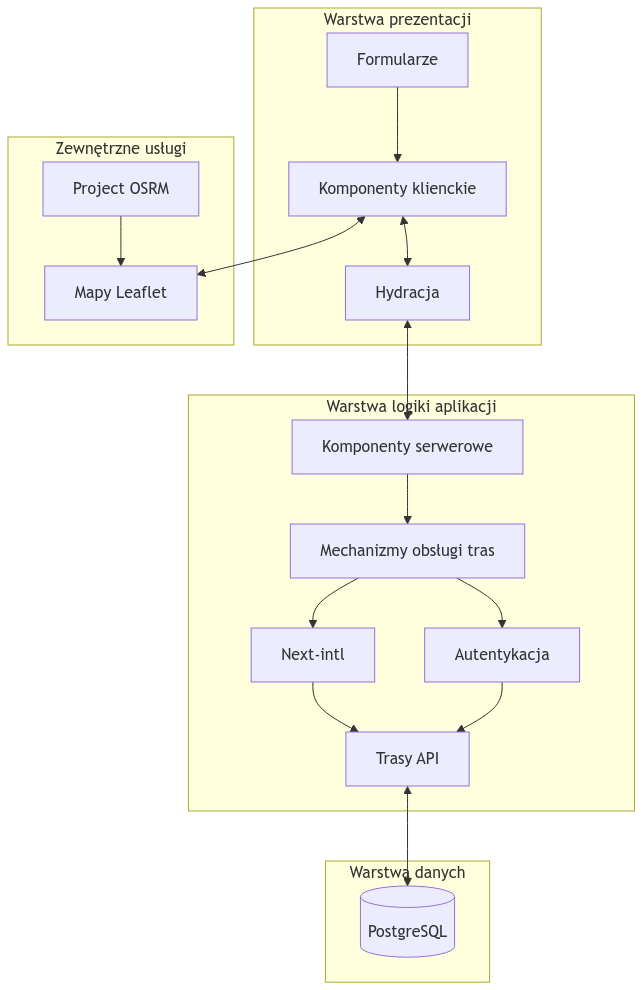
\includegraphics[width=0.7\linewidth]{rozdzial2/diagram_warstw.png}
	\caption{Diagram architektury warstw aplikacji}
	\label{Diagram warstw}
\end{figure}
To będzie kontynuowane